\section{Metodologia}
\label{sec:metodologia}

Para o cumprimento dos objetivos gerais e específicos do trabalho foram considerados catorze requisitos -- dez funcionais e quatro desejáveis -- pré-estabelecidos por um cliente fictício. Os requisitos estão listados abaixo:
\vspace{1 mm}

\textbf{Funcionais}
\begin{enumerate}
	\item Ser capaz de estabelecer comunicação com operador na superfície.
	\item Ser capaz de submergir e emergir de forma controlada.
	\item Ser capaz de se locomover em baixo d'água com uma velocidade de 2 m/s.
	\item Ser capaz de seguir trajetória pré-estabelecida.
	\item Ser capaz de mapear o leito submarino abaixo (angulação mínima de $ \pm $ 10°).
	\item Ser capaz de localizar no mapa um objeto pré-definido.
	\item Ser capaz de se deslocar até uma coordenada (3D) ou objeto pré-definido.
	\item Ser capaz de detectar ``sinal de socorro'' e se deslocar até a fonte emissora.
	\item Ser capaz de transmitir dados, inclusive a localização (3D) em tempo real.
	\item Ser capaz de armazenar o caminho percorrido para o cumprimento da missão.
\end{enumerate}

\textbf{Desejáveis}

\begin{enumerate}[resume]
	\item O protótipo deve suportar pressões correspondentes a pelo menos 10 mca.
	\item O protótipo deve ser ``bem montado'' e ``apresentável''.
	\item Deve-se preservar aspectos de segurança na operação, resgate e manutenção.
	\item Deve-se desenvolver IHM para monitoramento em tempo real.	
\end{enumerate}

\vspace{1 mm}

A metodologia adotada para levantamento de ideias, ponderação de requisitos e seleção preliminar de componentes está descrita na Figura \ref{fig:metodologia}. As subseções a seguir detalham o que foi desenvolvido em cada etapa da metodologia.

\begin{figure}[h]
	\centering
	\caption{Metodologia adotada para o projeto}
	\label{fig:metodologia}
	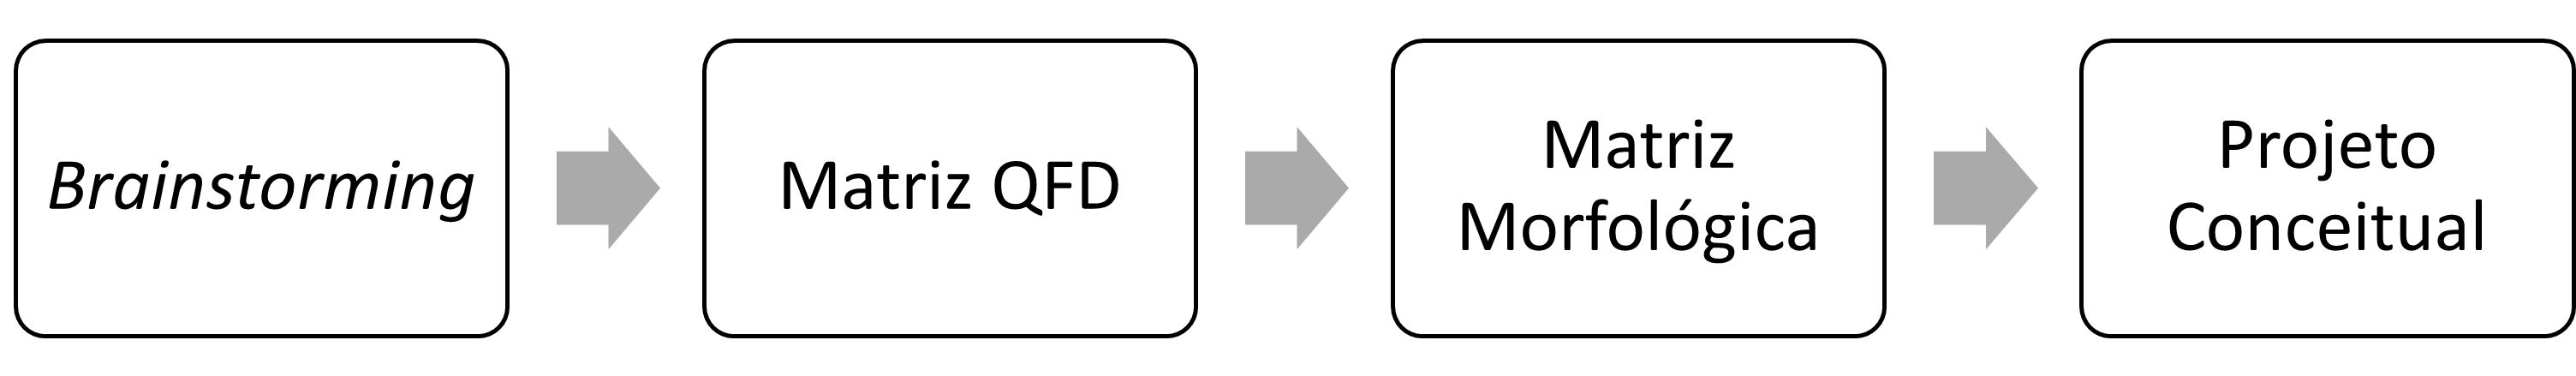
\includegraphics[width=0.7\linewidth]{images/metodologia}\\
	\footnotesize Fonte: Autores
\end{figure}

\subsection{\textit{Brainstorming}}
\label{subsec:brainstorming}

Na fase de \textit{brainstorming} foram levantadas algumas soluções que poderiam atender ao maior número possível de requisitos. Ao término dessa etapa, a equipe chegou a um conceito inicial, que está mostrado na Figura \ref{fig:conceito-inicial}.

\begin{figure}[h]
	\centering
	\caption{Conceito inicial da solução}
	\label{fig:conceito-inicial}
	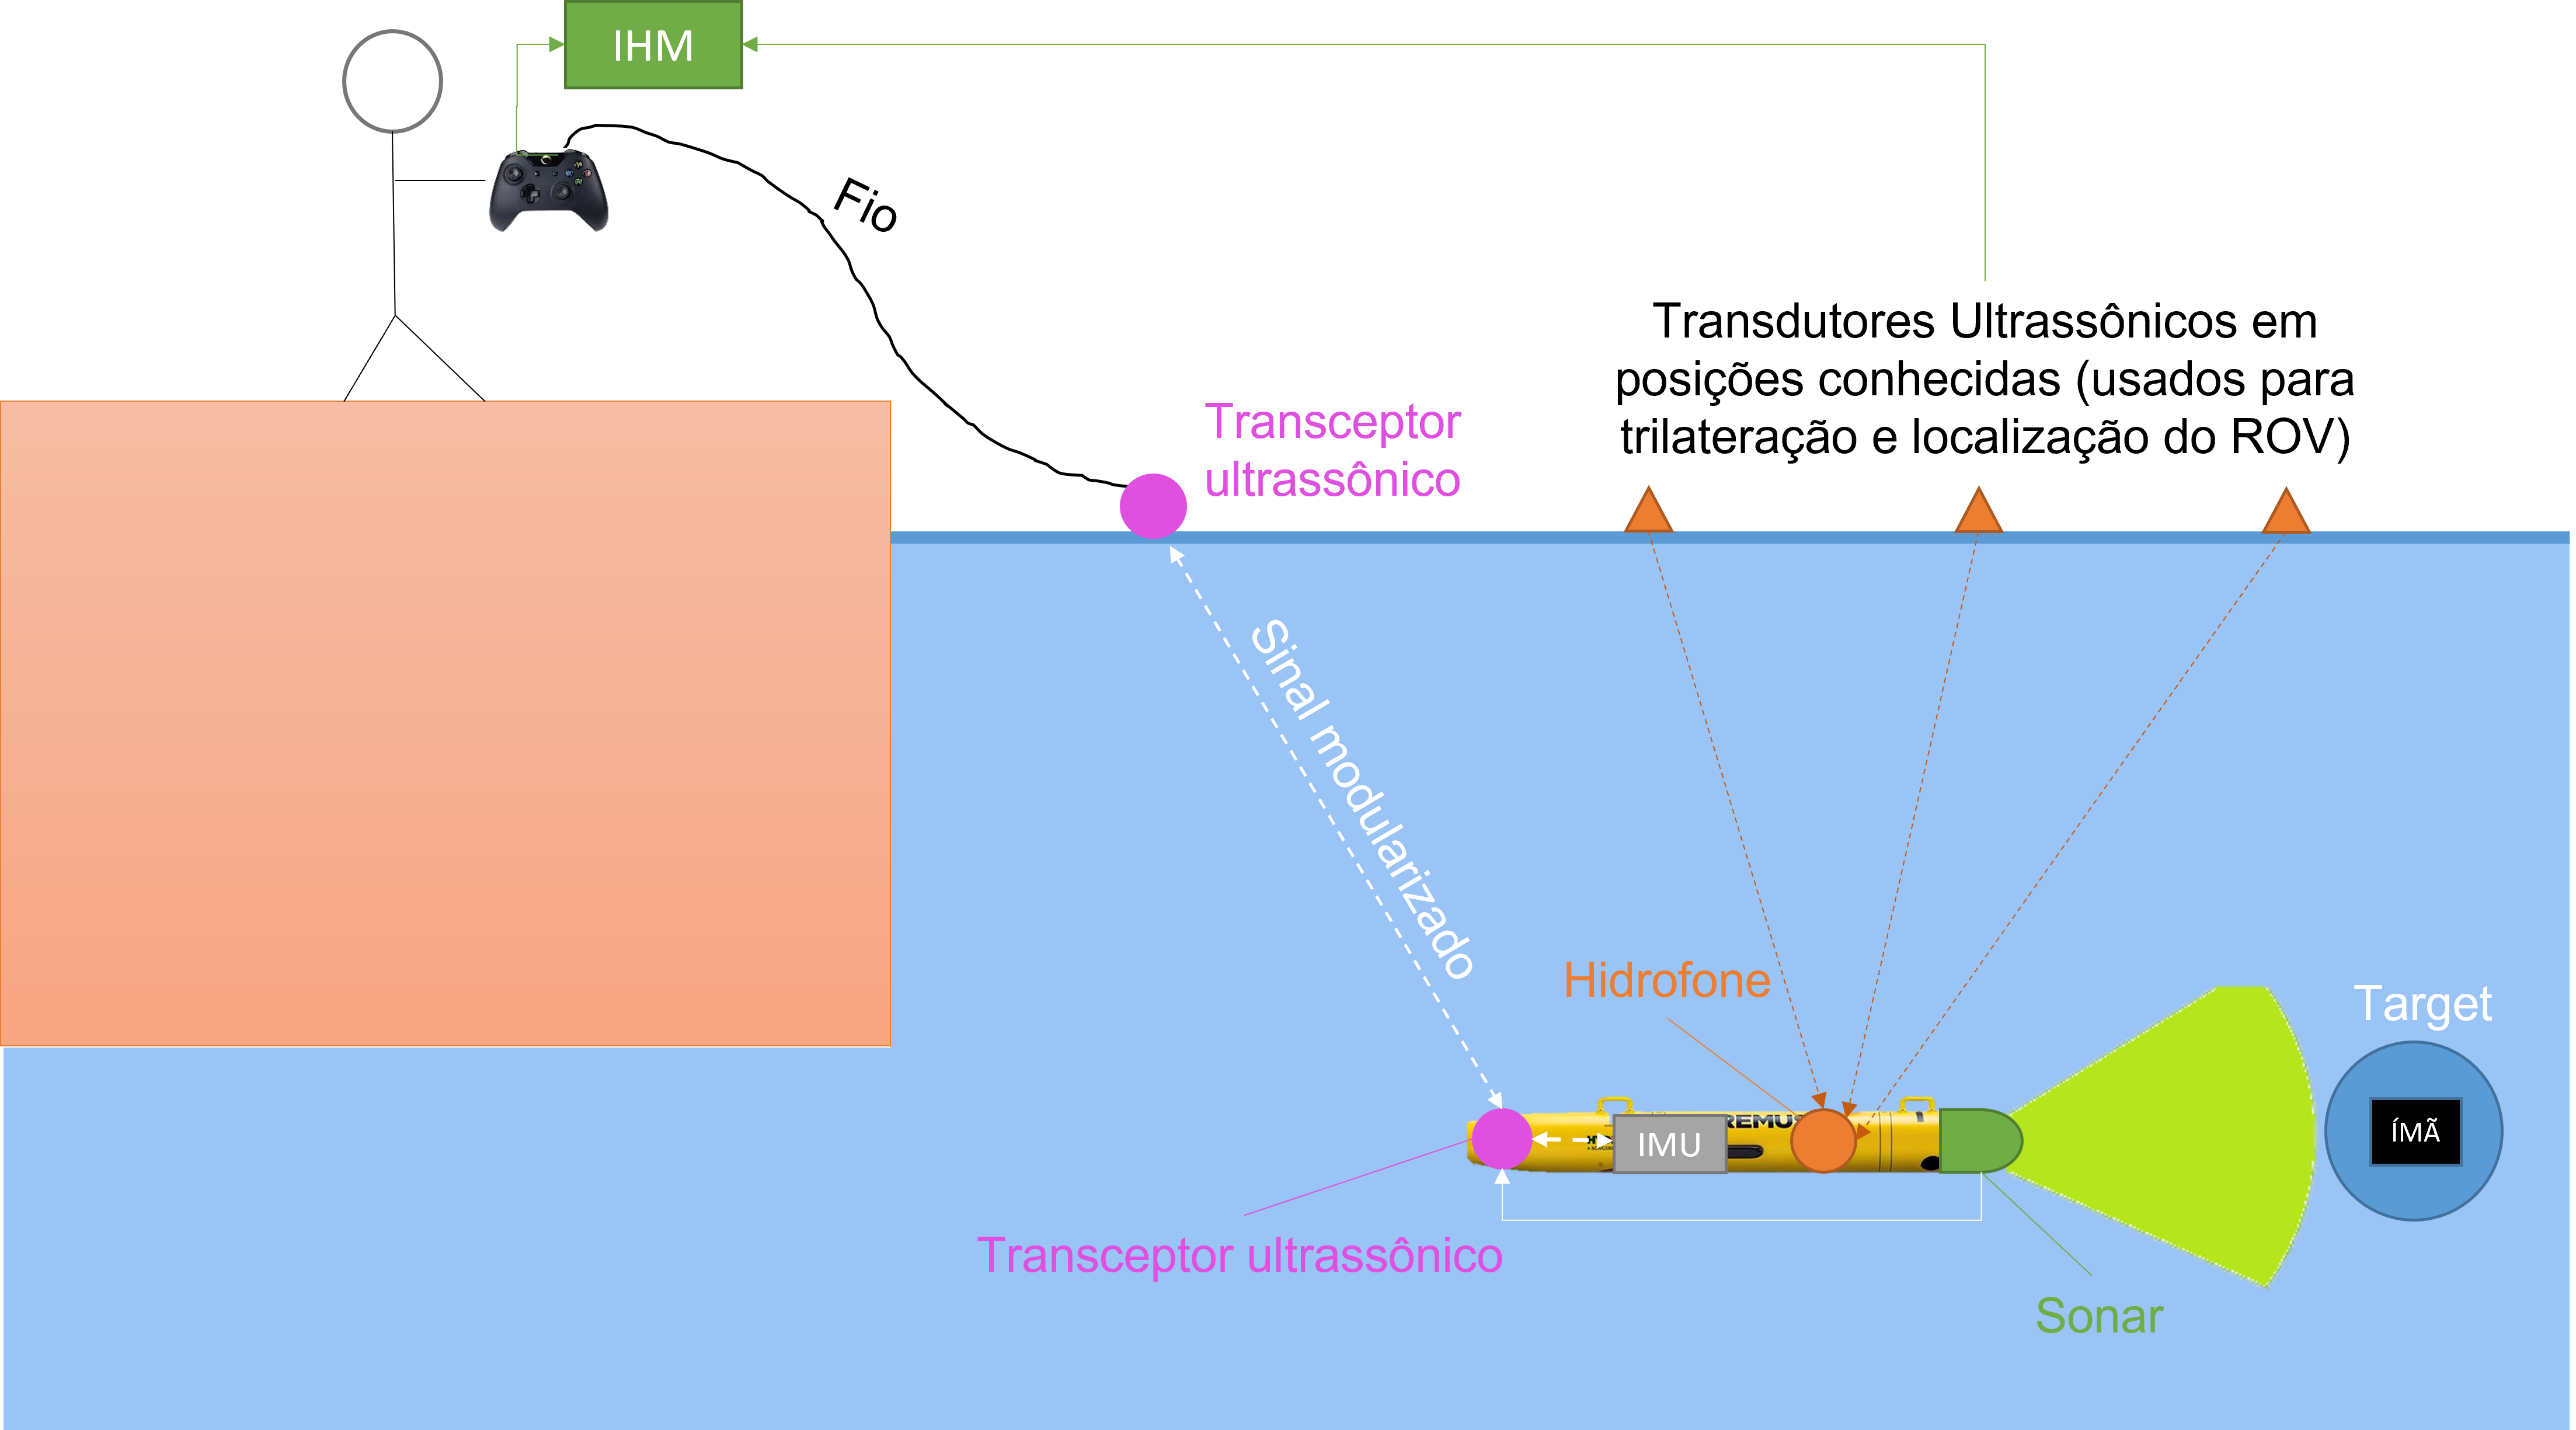
\includegraphics[width=1\linewidth]{images/conceito-inicial}\\
	\footnotesize Fonte: Autores
\end{figure}

Nesse conceito, o operador seria responsável por enviar comandos de deslocamento para um transceptor ultrassônico -- que estaria dentro de uma bóia na superfície -- através de um controle. O comando seria então convertido em um sinal modularizado para ser enviado ao transceptor ultrassônico presente no ROV. Em seguida, esse sinal seria decodificado e o ROV se deslocaria para a posição desejada. 

A localização do ROV seria periodicamente monitorada por três transdutores ultrassônicos presentes na superfície da água, que atuariam como \textit{ground-truth}, recebendo a informação de um hidrofone presente no ROV e calculando a localização por meio de trilateração. Essa informação seria então enviada para a inteface homem-máquina (IHM) via cabo ou RF.

A medida em que o ROV se aproximasse do objeto de interesse -- que estaria emitindo sinal acústico --, haveria uma amplificação do sinal do sonar embarcado, que seria transmitido para o transceptor ultrassônico presente no ROV e enviado de volta para o operador. O objeto teria também um ímã para facilitar a captura e resgate.

O mapeamento do leito seria feito de modo \textit{offline} por outro sensores ultrassônicos embarcados no ROV. O registro da trajetória também não seria feito em tempo real, mas de modo \textit{offline} por meio do rastro calculado pela IMU (do inglês \textit{Inertial Measurement Unit}).


\subsection{Matriz QFD}
\label{subsec:matriz-qfd}

Após obtenção de um conceito inicial, a equipe utilizou a Matriz QFD (do inglês \textit{Quality Function Deployment}) para conversão das necessidades do cliente fictício em requisitos factíveis de projeto. Nessa etapa foram avaliadas as relações entre as necessidades e os requisitos, assim como as correlações dos requisitos entre si. Não foi feita uma análise de concorrentes. Ao término do preenchimento da QFD, cujo recorte está mostrado na Tabela \ref{tab:qfd-brov-recorte}, foi possível determinar a ordem de priorização dos requisitos. Os principais requisitos listados foram:

\begin{enumerate}
	\item Comunicação \textit{wireless}.
	\item Localizar ROV.
	\item Seguir trajetória pré-estabelecida.
\end{enumerate}

\begin{table}[h!]
	\centering
	\caption{Matriz QFD}
	\label{tab:qfd-brov-recorte}
	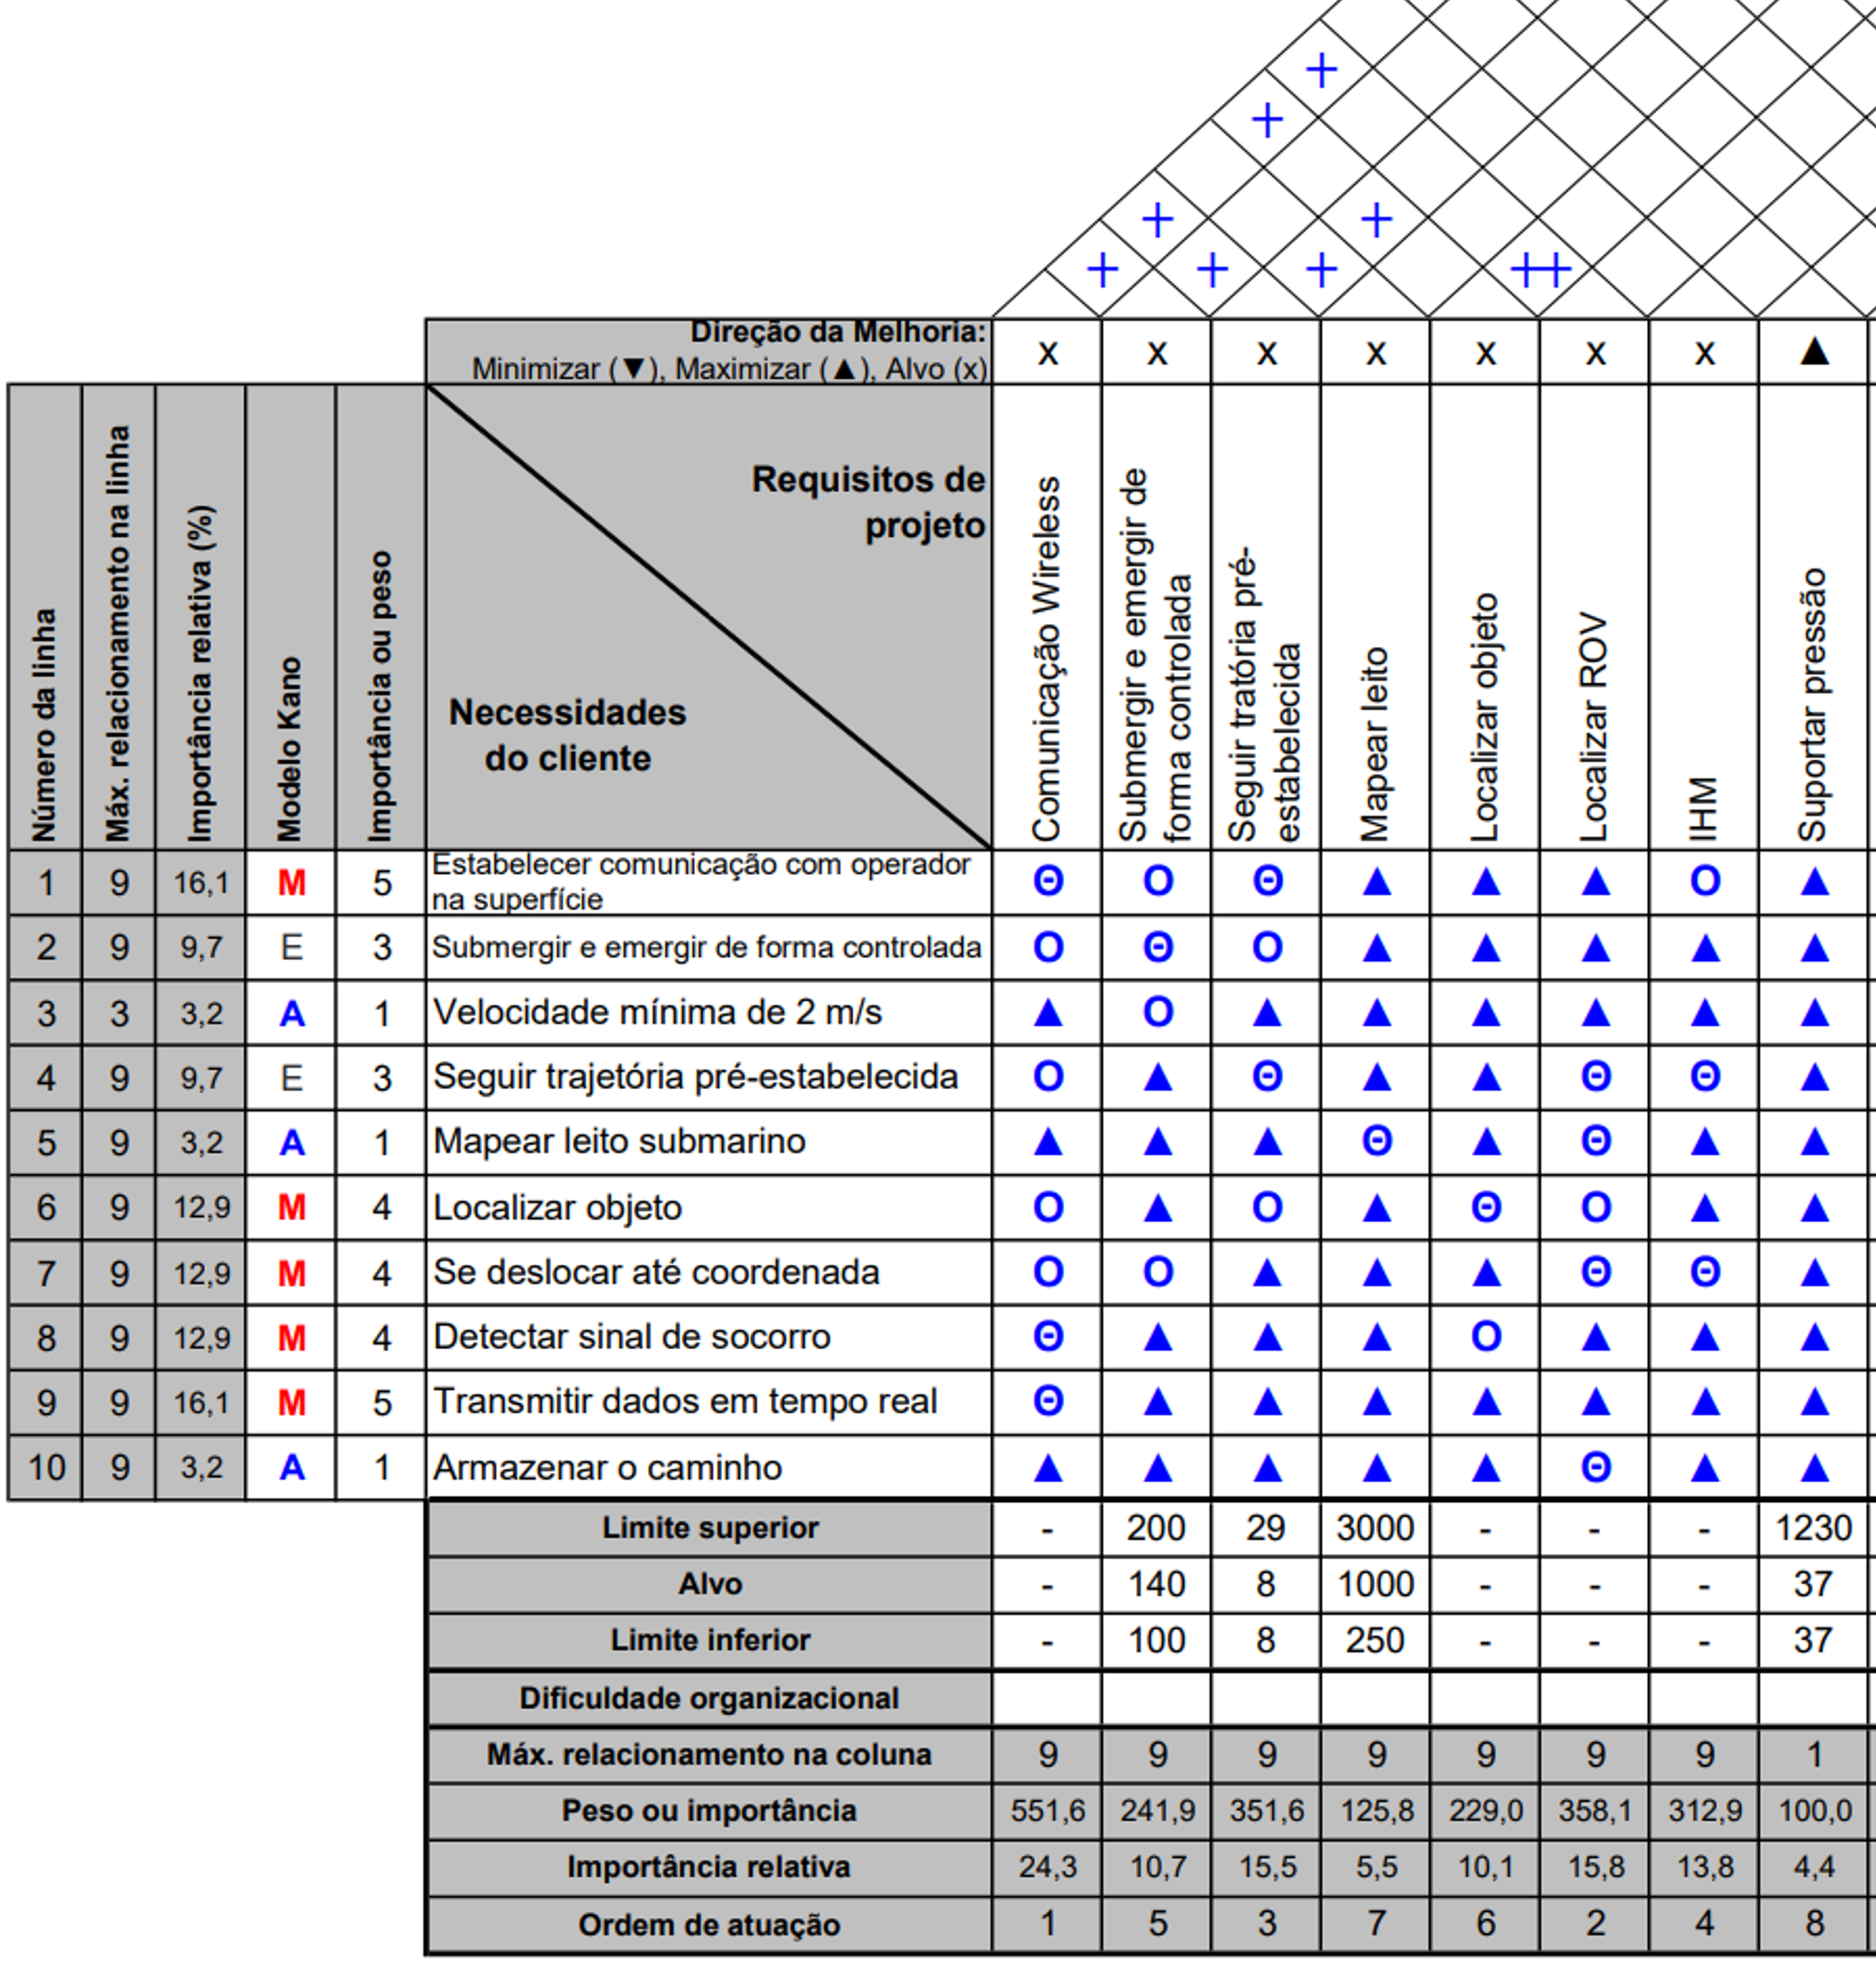
\includegraphics[width=1\linewidth]{images/QFD-BROV.png}\\
	\footnotesize Fonte: Autores
\end{table}

\subsection{Matriz Morfológica}
\label{subsec:matriz-morfologica}

A matriz morfológica, mostrada na Tabela \ref{tab:matriz-morfologica}, foi utilizada para seleção preliminar dos componentes e sistemas que viriam compor o ROV, de modo a solucionar cada requisito de projeto. Ao término do preenchimento da matriz morfológica, o conceito inicial sofreu alterações, como substituição e inclusão de novos sensores. Cada requisito de sistema foi convertido em um problema de engenharia e as soluções possíveis foram pesquisadas e escolhidas. Os argumentos para seleção de alguns dos componentes estão expostos a seguir.

\paragraph{Comunicação Wireless} em meio aquoso pode ser realizada de três formas: acústica, eletromagnética e óptica. Dentre essas formas, a acústica foi selecionada pois o atenuamento do sinal é menor do que as outras opções debaixo água. Além disso, a comunicação óptica apresenta restrição com alinhamento entre transmissor e receptor e a eletromagnética é fortemente atenuada na água, o que favorece mais a escolha da onda acústica, que não apresenta essas peculiaridades negativas.

\paragraph{Medição de Profundidade} vai ser realizada a partir da medição de sensor de pressão, que através de uma simples equação, pode ser convertida em profundidade. Essa alternativa foi escolhida visto a maior complexidade das outras alternativas: utilização de um transdutor para medição da distância da superfície da água e utilização de visão computacional e marcos fiduciais. Além de serem mais complexas, não apresentam grande melhoria em comparação com sensor de pressão.

\paragraph{Sistema de propulsão} pode ser composto por bombas de porão, motores de corrente contínua e motores \textit{brushless}. Os dois primeiros necessitam de conversores de corrente contínua para controle de velocidade, porém a resolução do conversor de corrente contínua é menor do que a resolução que se pode obter com os motores \textit{brushless}. Ademais, o motor \textit{brushless} consegue atingir velocidade maiores na mesma faixa de preço.

\paragraph{Controle de velocidade} do veículo pode-se usar diversas estratégias de controle, a escolhida pra ser adotada foi o controle multivariável baseado em modelo. Esse controlador foi escolhido pois permite controlar o empuxo em cada propulsor para se atingir a velocidade desejada, juntamente com a atenuação de grandes variações de velocidade do motor. 

\paragraph{Mapeamento de leito} utilizará sensores ultrassom de distância e a localização do veículo para geração de um mapa de ocupação 3D. Essa alternativa foi selecionada pela menor complexidade e custo das demais. Apesar de também ter menor qualidade, é o requisito que é o segundo menos importante de acordo com a Tabela \ref{tab:qfd-brov-recorte}, dessa forma, não é interessante gastar recurso financeiro de tempo para adotar uma técnica melhor.

\paragraph{Localização de objeto} vai contar com duas formas de localização. A primeira é a localização acústica com SBL (do inglês, \textit{Short BaseLine}), que através da trilateração estima a posição de um objecto no plano paralelo a superfície. A segunda é através de marcos fiduciais, que são adesivos com formado similares a um QR Code, o qual permite a estimação da pose de um objeto nos seis graus de liberdade. As duas serão utilizadas em conjunto pois são complementares. O SBL não fornece todos os graus de liberdade, mas consegue transmitir a direção do objeto para uma distância maior que a do marco artificial, que por sua vez estima todos os graus de liberdade de um objeto.

\paragraph{Localização do veículo} é o segundo requisito mais importante do projeto, por isso, com finalidade de ter um sistema preciso, diversas estratégias serão adotadas em conjunto. A localização do veículo consiste em saber a pose nos seis DOF (\textit{Degrees of Freedom}) do veículo em relação ao ambiente no qual está inserido. Para isso, o sistema SBL será usado para estimação da posição em XY, a medição de profundidade será usada para calcular o Z e o giroscópio para a orientação do veículo. Mesmo já sendo dessa forma possível obter a pose 6DOF do veículo com essas três soluções, a detecção de Arucos, \textit{dead-reckoning} e dados do acelerômetros também serão usados visando obtenção de uma localização mais precisa. 

\paragraph{Interface Homem Máquina} será realizada através do RVIZ. Essa escolha foi feita simplesmente pela compatibilidade de arquitetura de \textit{software}, visto que essa ferramenta é incorporada ao ROS (do inglês, \textit{Robotics Operating System}), que já será utilizado.

\paragraph{Estrutura} do veículo será tubular. Esse tipo de estrutura permite a fácil modificação do projeto, além de ter uma menor massa adicional, o que permite o melhor controle do veículo, como também a fácil modificação do projeto.

\begin{table}[h!]
	\centering
	\caption{Matriz morfológica}
	\label{tab:matriz-morfologica}
	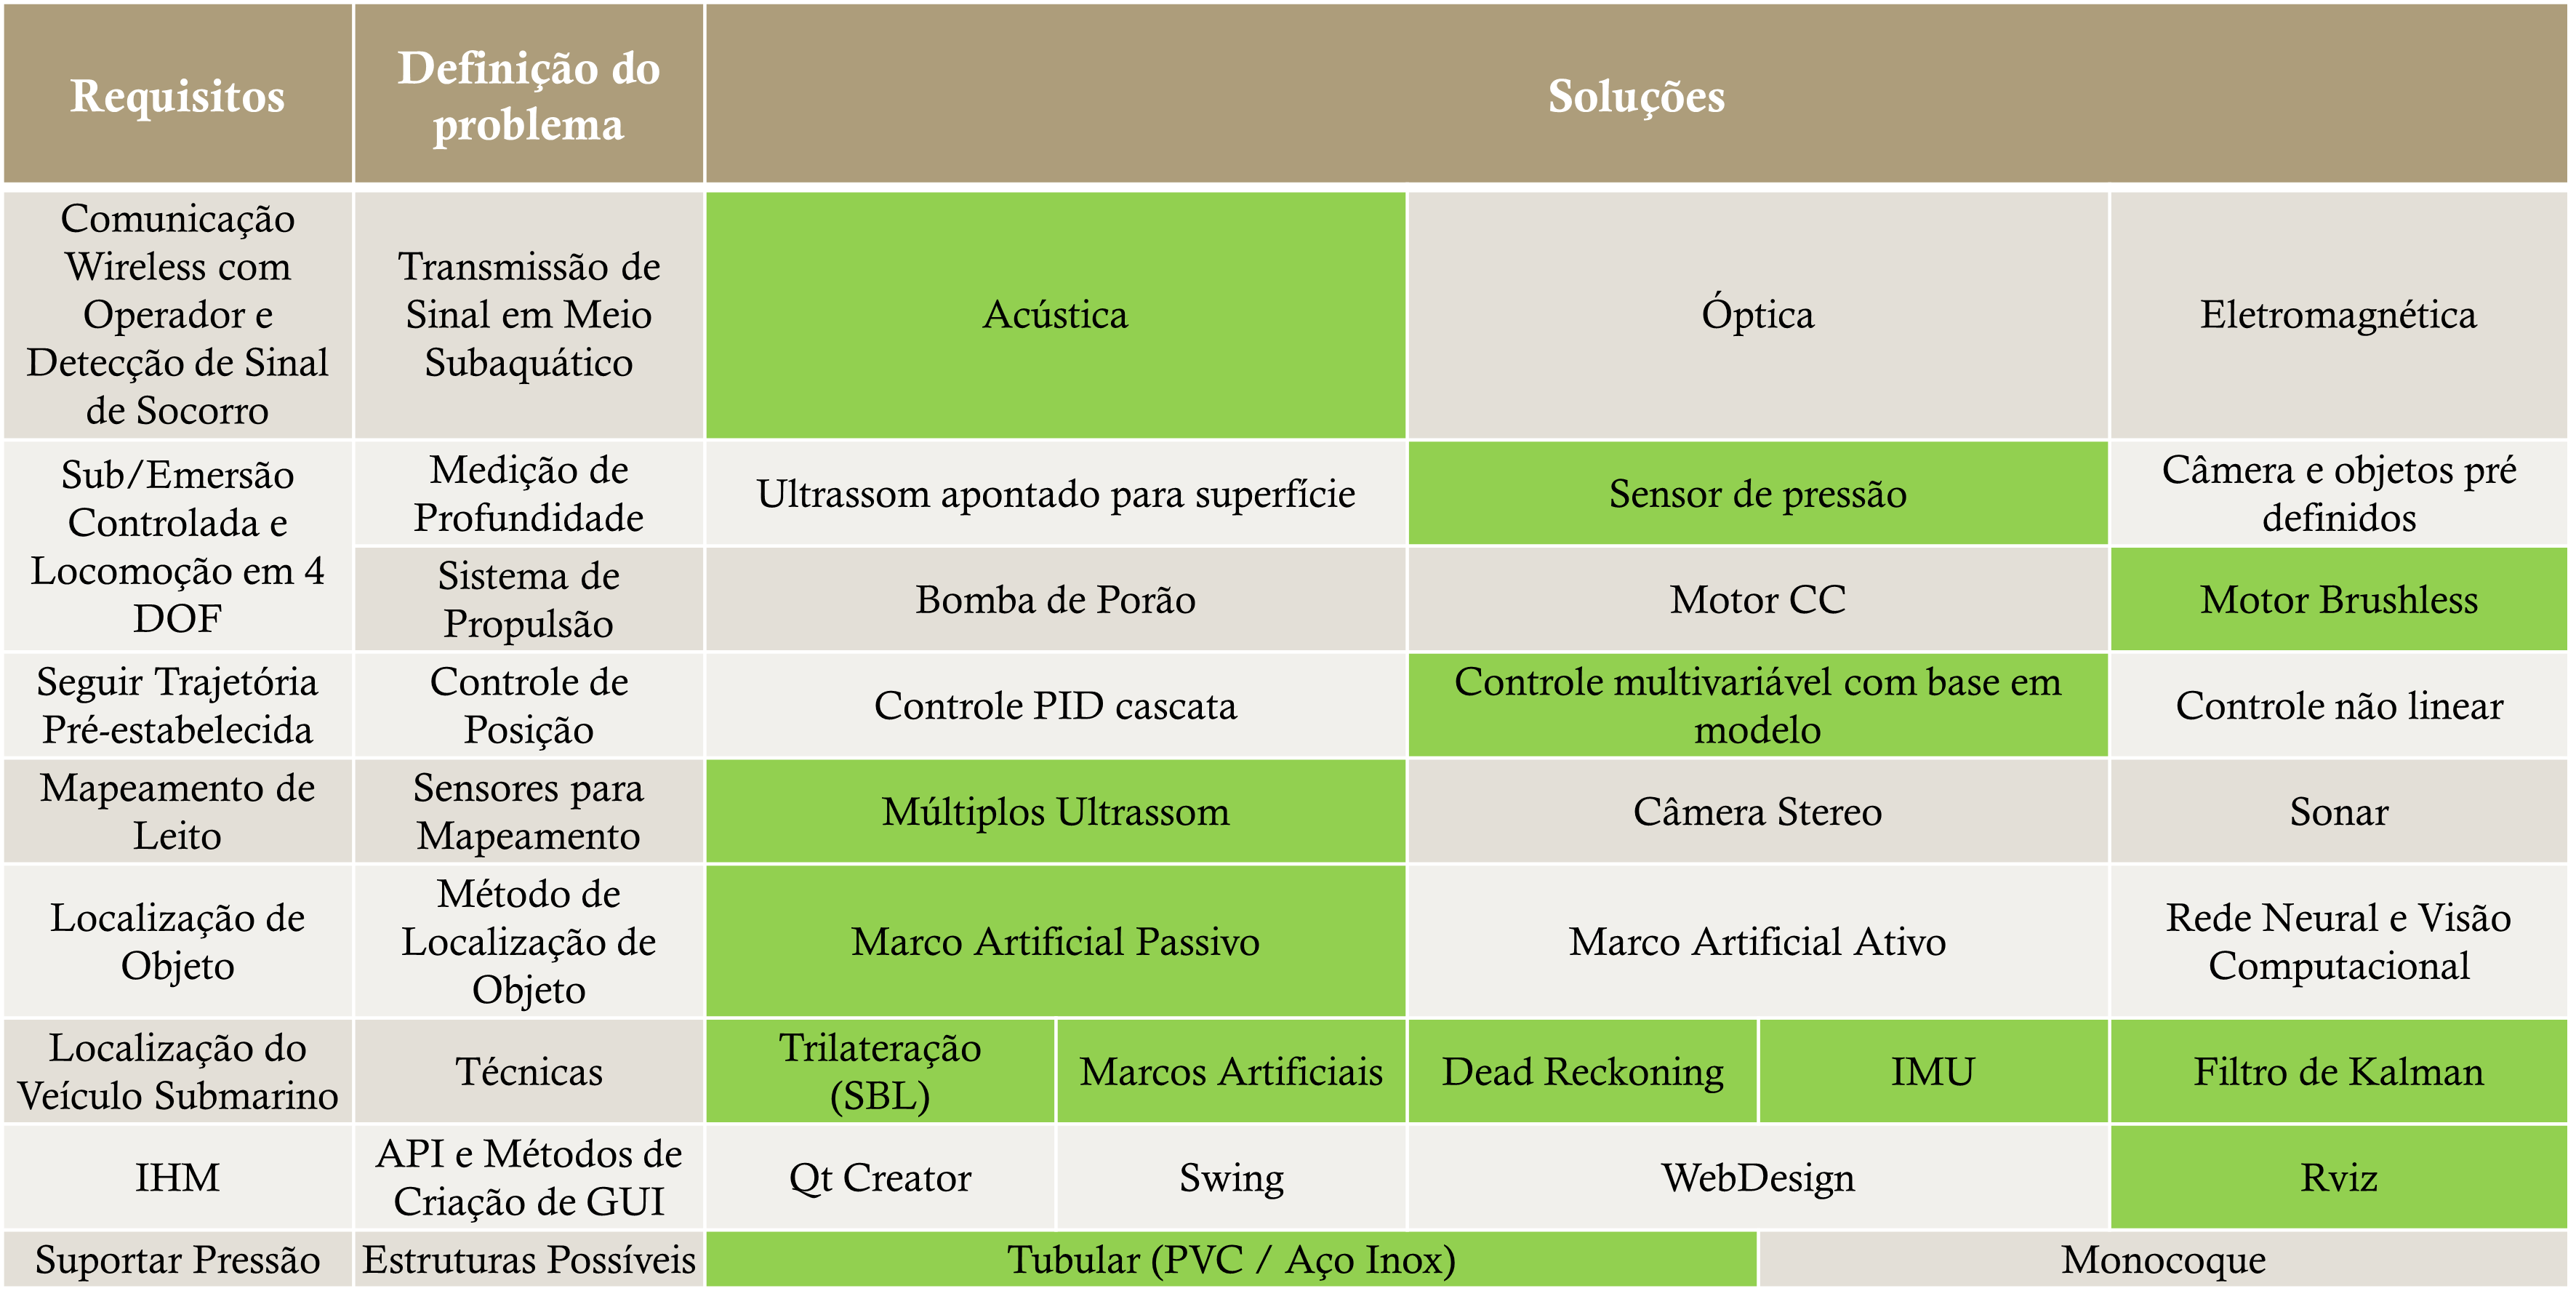
\includegraphics[width=1\linewidth]{images/Matriz-morfologica}\\
	\footnotesize Fonte: Autores
\end{table}

\subsection{Projeto Conceitual}
\label{subsec:projeto-conceitual}

Após as decisões de projetos tomadas a partir da matriz QFD e morfológica, o projeto conceitual resultante do \textit{brainstorm} passou por algumas modificações, que podem ser observadas na Figura \ref{fig:conceito-final}. Quanto aos sensores do veículo, o sonar foi substituído pela câmera, visto que é um recurso muito mais barato e atende a estimação da pose do objeto. O acréscimo de sensores ultrassom no fundo do veículo para mapeamento e o imã para possibilitar o resgate de uma moeda.

Na superfície, também modificou-se o módulo flutuante, que deve se comunicar sem fio tanto com o controle do operador, como com a IHM, não há necessidade de comunicação com fio. Além disso, o sistema SBL vai deixar de estar boiando, pois pode sair do lugar e gerar error no sistema de localização.  

\begin{figure}[h]
	\centering
	\caption{Conceito da solução após matriz morfológica}
	\label{fig:conceito-final}
	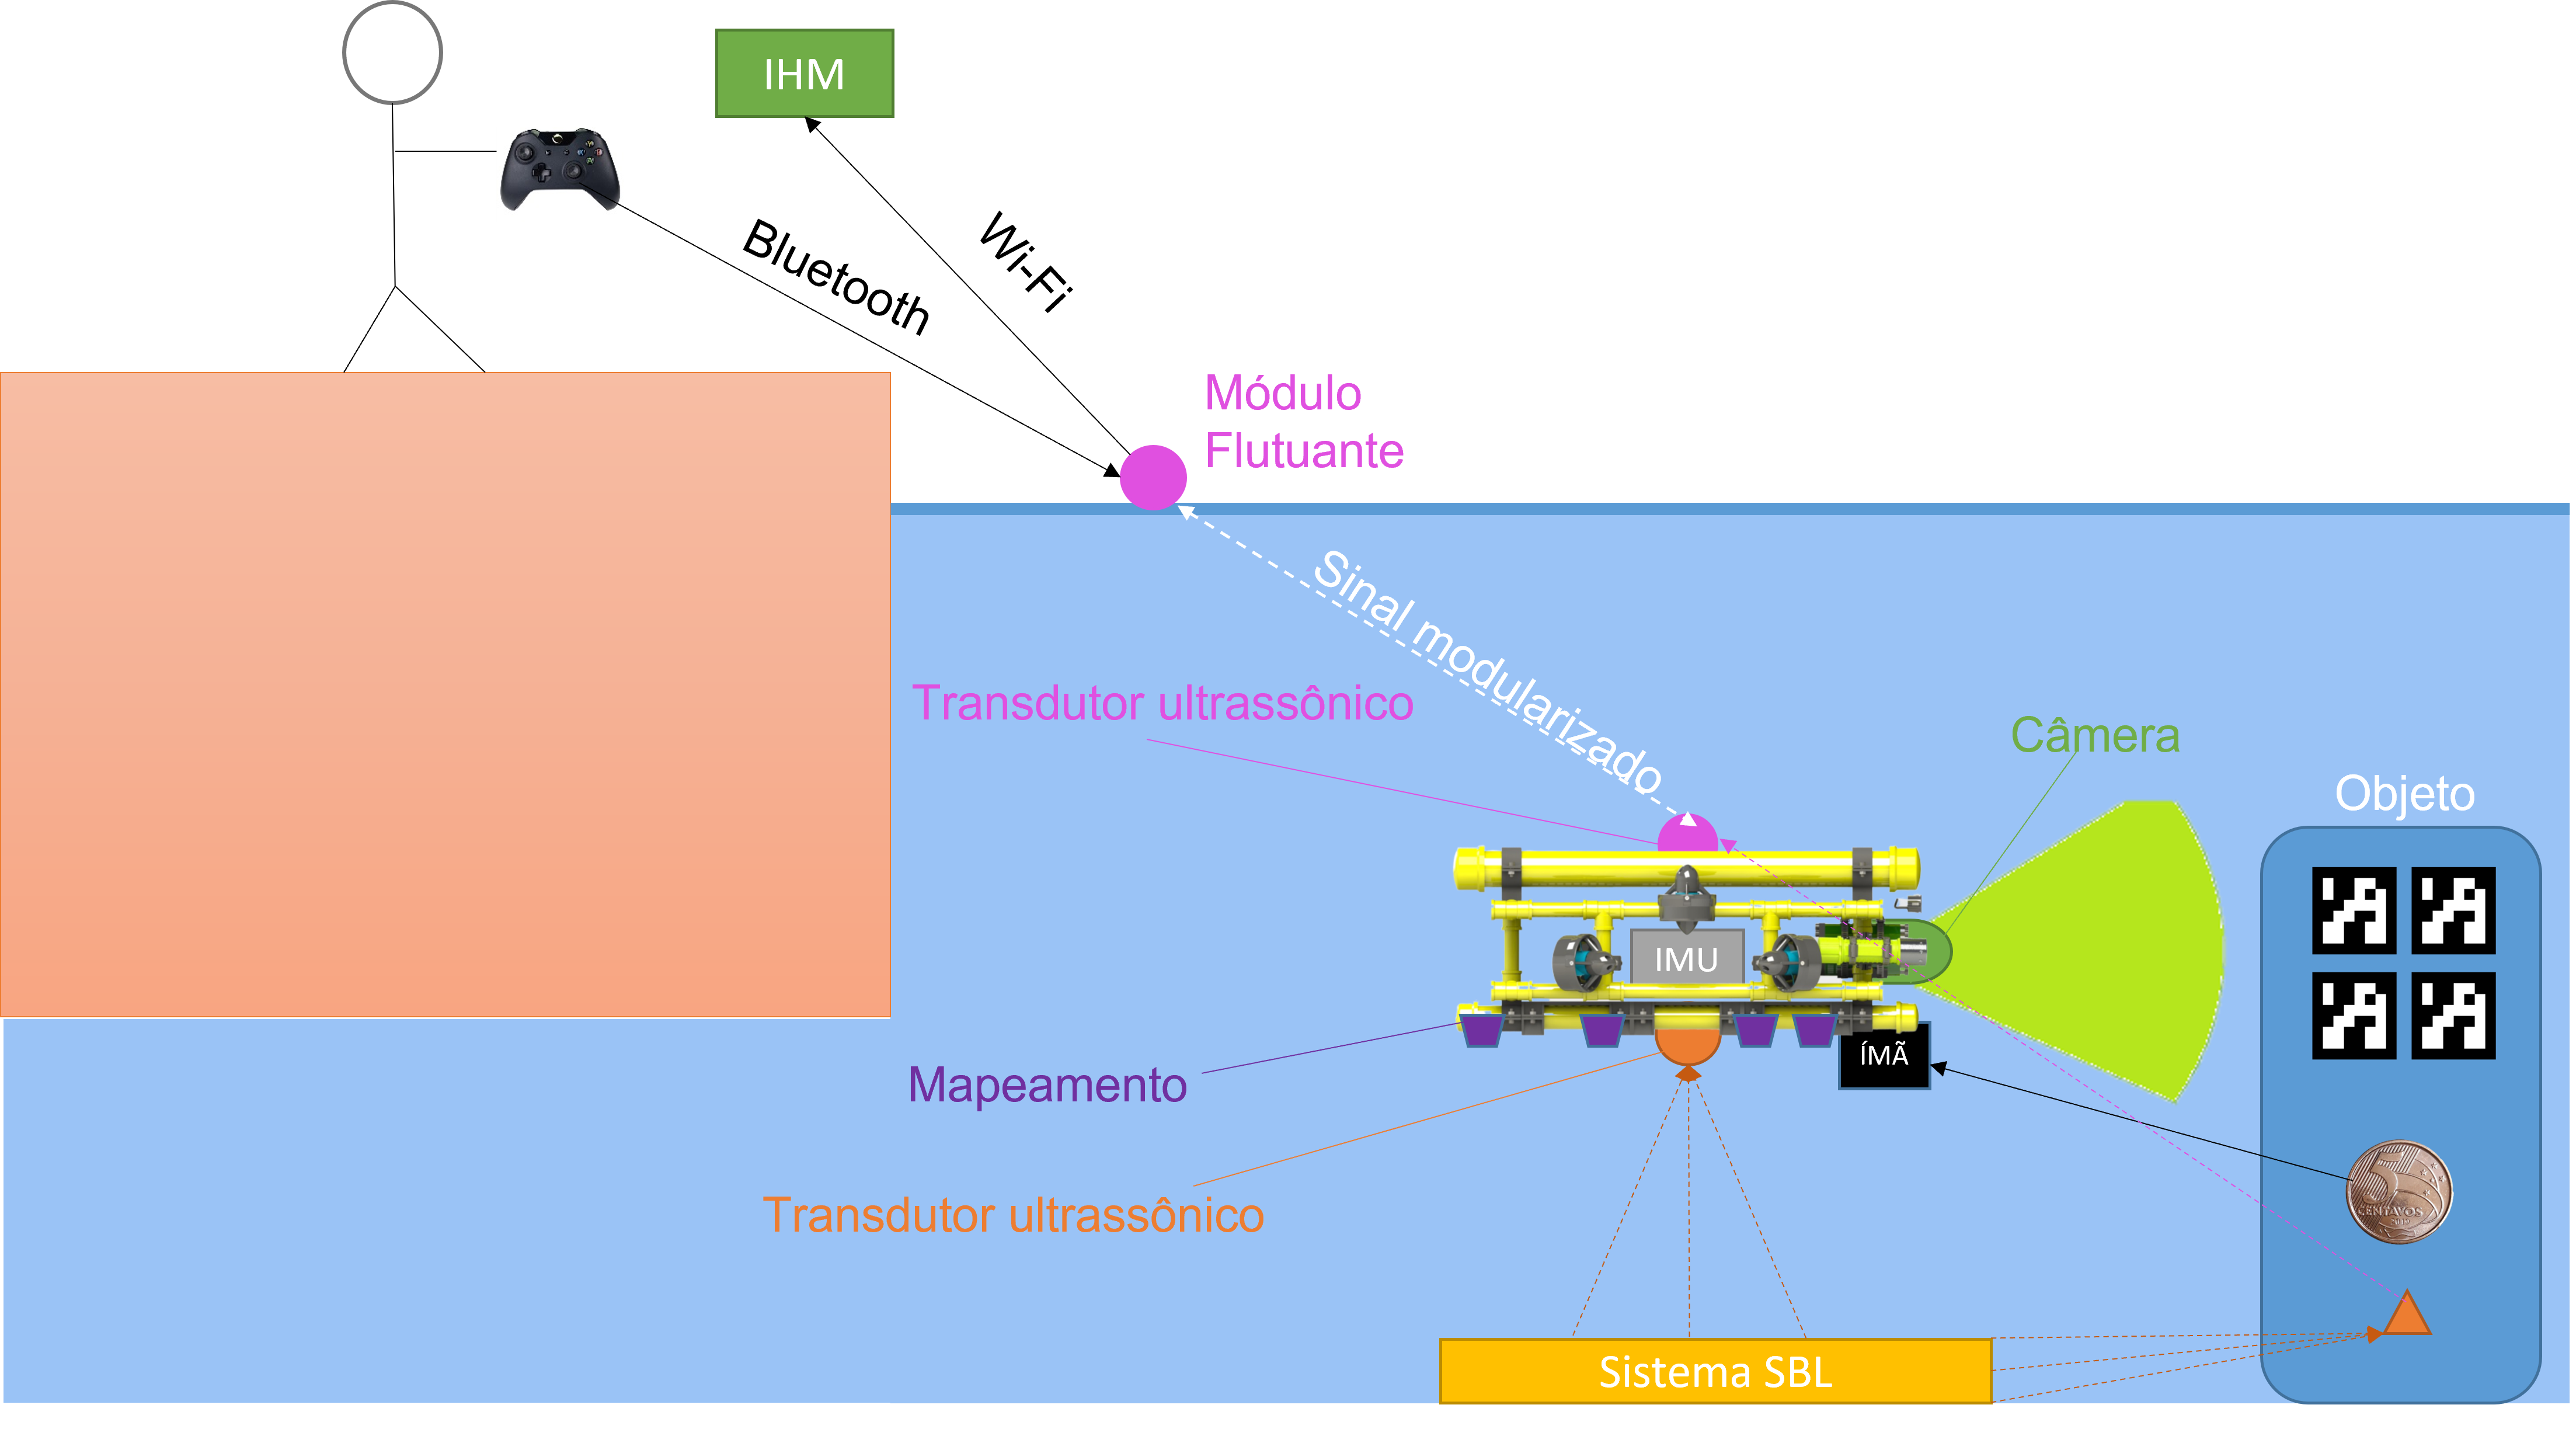
\includegraphics[width=1\linewidth]{images/conceito-final}\\
	\footnotesize Fonte: Autores
\end{figure}

Por fim, o objeto vai contar com uma moeda, um transdutor e marcos fiduciais. A moeda é simplesmente para comprovação de que o veículo se alcançou o objeto. O transdutor é para estimação da pose do objeto e transmissão dessa informação pro veículo. Por fim, os marcos fiduciais para fazer são para uma estimação mais precisa e com todos os graus de liberdade d veículo.
